% =====================================================================
%  hvrb_topology_v1.tex -- HVRB topology for the HVRB sheet (v3)
%  EXACT curves (closed forms on the sheet), no fitted data:
%   (a) lambda(phi) = 1 - (1 - phi^MR/XR)^XR, phi in [0, XR^(1/MR)]
%   (b) g(lambda) = MR XR^(1-1/MR) (1-lam)^(1-1/XR) [1-(1-lam)^(1/XR)]^(1-1/MR)
%  Curves: proposed Material X set MR = 1.5, XR = 2.5 (oiblue): peak at
%  lambda = 0.394, g_max = 0.854, phi_end = 1.842 (checked by script).
%  Contrast: MR = 1.5, XR = 1.0 (oivermil), the CTH input defaults
%  quoted in SAND2025-09228 Sec. 3.2: g rises to lambda = 1 and the burn
%  ends abruptly at phi = 1.  Both solid (both exact).
% =====================================================================
\documentclass[border=2pt]{standalone}
\usepackage{pgfplots}
\pgfplotsset{compat=1.15}
\definecolor{slate}{HTML}{2C3E50}
\definecolor{oiblue}{HTML}{0072B2}
\definecolor{oivermil}{HTML}{D55E00}
\begin{document}
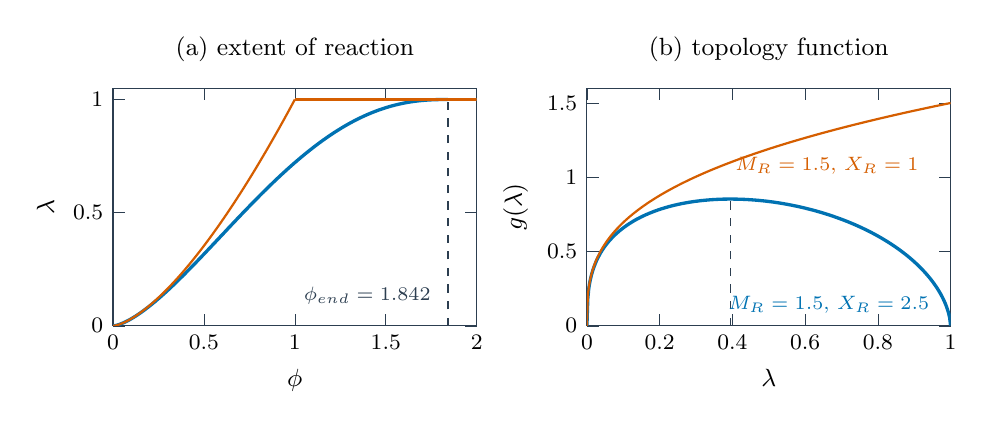
\begin{tikzpicture}
\pgfplotsset{every axis/.style={width=6.2cm,height=4.6cm,axis line style={slate},tick style={slate},
  label style={font=\small},tick label style={font=\footnotesize},samples=400}}
\begin{axis}[name=a,xmin=0,xmax=2,ymin=0,ymax=1.05,xlabel={$\phi$},ylabel={$\lambda$},
  title={\small (a) extent of reaction}]
  \addplot[oiblue,very thick,domain=0:1.842] {1-(1-x^1.5/2.5)^2.5};
  \addplot[oiblue,very thick,domain=1.842:2,forget plot] {1};
  \addplot[oivermil,thick,domain=0:1] {x^1.5};
  \addplot[oivermil,thick,domain=1:2,forget plot] {1};
  \draw[slate,dashed,thin] (axis cs:1.842,0) -- (axis cs:1.842,1);
  \node[font=\scriptsize,slate,anchor=south east] at (axis cs:1.80,0.05) {$\phi_{end}=1.842$};
\end{axis}
\begin{axis}[at={(a.east)},anchor=west,xshift=1.4cm,xmin=0,xmax=1,ymin=0,ymax=1.6,
  xlabel={$\lambda$},ylabel={$g(\lambda)$},title={\small (b) topology function}]
  \addplot[oiblue,very thick,domain=0:0.99999] {1.5*2.5^(1-1/1.5)*(1-x)^(1-1/2.5)*(1-(1-x)^(1/2.5))^(1-1/1.5)};
  \addplot[oivermil,thick,domain=0:1] {1.5*x^(1-1/1.5)};
  \draw[slate,dashed,thin] (axis cs:0.394,0) -- (axis cs:0.394,0.854);
  \node[font=\scriptsize,text=oiblue] at (axis cs:0.665,0.14) {$M_R=1.5$, $X_R=2.5$};
  \node[font=\scriptsize,text=oivermil,anchor=north] at (axis cs:0.66,1.20) {$M_R=1.5$, $X_R=1$};
\end{axis}
\end{tikzpicture}
\end{document}
